% Camera-ready ICAIF '26 — ACM sigconf (aceito; TAPS; limite 9 p. com referências).
% Fonte do corpo: projects/p1_deterrence/chapters/icaif26.md via
%   make paper PROJECT=p1_deterrence VENUE=icaif26
\documentclass[sigconf]{acmart}
\citestyle{acmauthoryear}

% Bloco de direitos: copiado literalmente do e-mail do ACM e-Rights
% (rightsreview@acm.org, 2026-10-13). Não editar — o TAPS valida contra ele.
% Requer acmart >= 1.86 (\setcctype); o build local usa shared/latex/acmart/.
\copyrightyear{2026}
\acmYear{2026}
\setcopyright{cc}
\setcctype{by}
\acmConference[ICAIF '26]{7th ACM International Conference on AI in Finance}{November 14--17, 2026}{Milan, AA, Italy}
\acmBooktitle{7th ACM International Conference on AI in Finance (ICAIF '26), November 14--17, 2026, Milan, AA, Italy}
\acmDOI{10.1145/3858063.3858865}
\acmISBN{979-8-4007-3087-0/2026/11}



% Suporte aos fragmentos gerados pelo pandoc
\providecommand{\tightlist}{\setlength{\itemsep}{0pt}\setlength{\parskip}{0pt}}
\providecommand{\pandocbounded}[1]{#1}
\providecommand{\real}[1]{#1}
\graphicspath{{./}}
\setkeys{Gin}{width=\linewidth,keepaspectratio}

% (\acmConference vem do bloco de direitos acima)

% CCS — IDs conferidos no SKOS oficial da ACM (acm_ccs2012) em 2026-10-13;
% ver process/camera_ready_icaif26/ccs_auditoria.md.
\begin{CCSXML}
<ccs2012>
   <concept>
       <concept_id>10010147.10010257.10010258.10010261.10010275</concept_id>
       <concept_desc>Computing methodologies~Multi-agent reinforcement learning</concept_desc>
       <concept_significance>500</concept_significance>
       </concept>
   <concept>
       <concept_id>10003752.10010070.10010099.10010102</concept_id>
       <concept_desc>Theory of computation~Solution concepts in game theory</concept_desc>
       <concept_significance>300</concept_significance>
       </concept>
   <concept>
       <concept_id>10010405.10010455.10010460</concept_id>
       <concept_desc>Applied computing~Economics</concept_desc>
       <concept_significance>300</concept_significance>
       </concept>
   <concept>
       <concept_id>10010405.10010455.10010458</concept_id>
       <concept_desc>Applied computing~Law</concept_desc>
       <concept_significance>100</concept_significance>
       </concept>
 </ccs2012>
\end{CCSXML}

\ccsdesc[500]{Computing methodologies~Multi-agent reinforcement learning}
\ccsdesc[300]{Theory of computation~Solution concepts in game theory}
\ccsdesc[300]{Applied computing~Economics}
\ccsdesc[100]{Applied computing~Law}

\title{Algorithmic Collusion Without Deterrence: Auditing the Punishment Mechanism in Q-Learning Pricing Agents}

\author{Kau\^{e} Lopes de Moraes}
\affiliation{%
  \institution{University of S\~{a}o Paulo}
  \city{S\~{a}o Paulo}
  \country{Brazil}}
\email{kaue.moraes@usp.br}

\author{Rodrigo De Losso}
\affiliation{%
  \institution{University of S\~{a}o Paulo}
  \city{S\~{a}o Paulo}
  \country{Brazil}}
\email{delosso@usp.br}

\begin{document}

\begin{abstract}
Independent tabular Q-learning agents repricing in a simulated Bertrand
duopoly converge to supracompetitive prices, and the seminal evidence
attributes this to a learned reward--punishment scheme: undercut your
rival and it retaliates, so deviation never pays. This mechanistic
reading is what turns high prices into a cartel, and into a regulatory
target. We replicate the environment of \citet{calvano2020} and confirm
their impulse-response pattern within co-trained pairs. We then audit
the pattern on frozen policies, with learning off, and find that on its
own it does not identify a mechanism: the return is over-determined
rather than selective. Seventeen of eighteen converged pairs have a
single attractor whose basin is the entire state space, so every
perturbation returns whatever provoked it, and a forced price
\emph{increase} triggers the same retaliatory pattern as an undercut.
What co-training produces is a narrow, dyad-specific basin of
attraction: re-match frozen agents from independent runs, as Calvano et
al.~did with learning on, and coordination collapses by 81\% with
nothing carried across. The deterrence claim is incomplete on its own
terms: the one-period undercut of Calvano et al.'s impulse-response test
is unprofitable, which we confirm in every pair, but the \emph{optimal}
deviation, computed by dynamic programming against each partner's frozen
strategy, profits by 14.8\% on average. The scheme deters only the
deviation no optimizer would choose; collusion survives because
deviation is never tried, not because it would not pay. Supracompetitive
prices are robust; the punishment mechanism read into them does not
survive these tests, which changes what the standard test of algorithmic
collusion establishes, and what pairing-disruption remedies can be
expected to do.

\begin{center}\rule{0.5\linewidth}{0.5pt}\end{center}
\end{abstract}

\keywords{algorithmic collusion, multi-agent reinforcement learning, Q-learning, algorithmic pricing, market simulation, antitrust}

\maketitle

\section{Introduction}\label{introduction}

A growing literature reports that simple reinforcement-learning agents,
trained independently in repeated pricing games, converge to prices well
above the static Nash equilibrium. The seminal contribution of
\citet{calvano2020} goes further than documenting supracompetitive
prices: it offers a mechanism. After a forced unilateral price cut, the
rival's price drops and both prices then return to their pre-deviation
level, a pattern the authors read as a ``reward--punishment scheme''
that stabilizes the collusive outcome. This mechanistic reading is what
gives the result its policy weight: prices that are merely high are an
artifact; prices \emph{defended by retaliation} are a cartel.

This paper asks a narrow question with broad consequences: \textbf{is
there actually a punishment mechanism?} We take the question seriously
on Calvano et al.'s own terms. We replicate their environment and their
impulse-response experiment, and we confirm their pattern: within
co-trained pairs, the deviation-drop-return dynamic is robust (Section
4.2). The contribution builds on a line of work that has questioned
parts of the mechanistic reading with separate instruments (Section 2),
and it is twofold. The negative half is a five-part audit of the
mechanism behind the pattern (Section 4.3) and an incentive accounting
of the converged play (Section 4.5), run jointly on the same frozen
policies: taken on its own terms, the exhibit does not establish
deterrence. The positive half is what we find in its place: co-training
produces a \emph{dyad-specific basin of attraction}, a joint object
carved by the pair and without value outside it. The direct test takes
the rematching exercise of \citet[Section VI.B]{calvano2020} and turns
it into an evaluation protocol: re-match converged agents across
independent training runs with learning off, and coordination collapses
by 81\% (Section 4.4). Throughout, the design separates the
\emph{learning phase} from the \emph{measurement phase}: in the language
of experimental economics, Calvano et al.~evaluate in the partner
treatment, and we add the stranger treatment as a test rather than as a
re-training exercise (Section 3.1).

None of the five audits finds a punishment mechanism. The retaliatory
response fires for \emph{any} off-path price, including a cooperative
price increase; faced with an opponent that actually punishes, the
agents undercut it and absorb the permanent punishment rather than
sustain the cooperative path it offers; the learned reaction functions
are uncorrelated with best-response logic; the celebrated
return-to-baseline is forced by the geometry of the converged policies,
which have a single global attractor, so it would follow any
perturbation; and none of this reflects a representational limit,
because hand-built punishment rules fit the same policy matrix exactly.
What survives the audit is real but different in kind: a locally
calibrated, dyad-specific basin of attraction, fast to return, blind to
why it was perturbed, and specific to the pair that carved it.
Deterrence is a property an agent has; what training built here is a
property only the pair has.

We are careful about what we do \emph{not} claim. Calvano et al.~report
that about half of their sessions reach an on-path Nash equilibrium of
the repeated game, with small one-step losses elsewhere, and rarely a
subgame-perfect one; we do not dispute these statistics, and Section 4.5
says how our best-response measure relates to theirs. Our target is the
mechanistic interpretation, the ``reward--punishment scheme,'' in the
sense that matters for economics: a scheme, in the tradition of
\citet{friedman1971} and \citet{abreu1988}, is a rule that
\emph{enforces a prescribed path}. It responds to departures from that
path, and it sustains the path because the response makes deviating
unprofitable. That enforcement structure is what the audits do not find.

\section{Background}\label{background}

\textbf{Punishment schemes.} The language of ``reward--punishment
schemes'' carries a precise meaning in repeated-game theory. In
\citet{friedman1971}, collusion is sustained by a trigger strategy:
cooperate until anyone defects, then revert to static Nash forever.
\citet{abreu1988} generalizes this to optimal penal codes, in which
deviations, including deviations from the punishment itself, restart a
calibrated punishment phase. Two features are constitutive. First,
\emph{path enforcement}: the scheme prescribes a path and responds to
departures from it, in order to make deviating unprofitable. Second,
\emph{incentive compatibility}: the threat is credible because carrying
it out is optimal given the scheme (under imperfect monitoring,
punishment can even fire without any deviation; \citet{green1984}). Our
audit therefore does not ask whether the learned response fires only
after defections (a trigger rule need not be selective in that sense)
but whether the response has the \emph{structure} of path enforcement
(Sections 4.3(i)--(iii)), whether the enforced path is
incentive-compatible (Section 4.5), and whether the return itself is
selective at all, or forced by the structure of the state space (Section
4.3(iv)).

\textbf{The \citet{calvano2020} result.} Two firms in a logit-Bertrand
duopoly simultaneously choose prices from a 15-point grid; demand is
\(q_i = e^{(a_i-p_i)/\mu} / \big(\sum_j e^{(a_j-p_j)/\mu} + e^{a_0/\mu}\big)\)
and profit is \(\pi_i = (p_i - c)\,q_i\), with \(a=2\), \(c=1\),
\(\mu=0.25\), \(a_0=0\). Each agent runs tabular Q-learning
\citep{watkins1992} on the state \(s_t = (p^A_{t-1}, p^B_{t-1})\) (225
states) with \(\alpha = 0.15\), \(\delta = 0.95\), and
\ensuremath{\varepsilon}-greedy exploration decaying geometrically to
zero. After convergence, prices settle well above Nash. We measure this
with the collusion index
\(\mathrm{CI} = (\bar{p}^{RL} - p^{NE})/(p^{M} - p^{NE})\), where
\(p^{NE} \approx 1.473\) and \(p^{M} \approx 1.925\). Calvano et al.'s
impulse-response analysis (force one agent to undercut for one period;
the rival's price falls and both then recover) is the exhibit read as a
``reward--punishment scheme,'' and it is what elevated the result to a
landmark for competition policy.

\textbf{Subsequent literature and the gap.} \citet{klein2021} finds
supracompetitive outcomes under sequential pricing, sensitive to
action-space granularity. \citet{asker2024} show that, for myopic
agents, counterfactual (``synchronous'') updating drives prices to the
competitive level, so that high prices stem from what the learning
protocol fails to evaluate rather than from strategy; \citet{hansen2021}
obtain supracompetitive prices from bandit algorithms with \emph{no}
punishment capability, and \citet{abada2023} reach a similar
exploration-based diagnosis. Empirically, algorithmic pricing changes
price competition \citep{brown2023, assad2024}; the regulatory stakes
are drawn out by \citet{harrington2018} and \citet{oecd2017}. Closest to
us, \citet[hereafter Calvano IJIO]{calvano2023} verify approximate
incentive compatibility on converged profiles and classify the 2020
environment's collusion as largely ``genuine.'' The interpretation has
since been examined from several directions, each with its own
instrument. \citet{epivent2024} show, in the same environment, that the
price war follows price \emph{hikes} as well as cuts, so the response
does not distinguish the direction of the deviation. \citet{denboer2022}
show that the impulse-response pattern (the rival cuts, prices return,
the deviation does not pay) can be generated by strategy profiles that
are neither equilibria nor reward--punishment schemes, and conclude that
a systematic test would have to check every unilateral deviation; they
carry this out exhaustively for two prices, and the 15-price case is
beyond enumeration. \citet{banchio2022} describe a mechanism that
sustains supracompetitive prices without any punishment: correlated
estimation errors across co-learning agents, which they call spontaneous
coupling. And \citet[Section VI.B]{calvano2020} themselves rematch
converged agents with learning still on: profit gains fall from 85\% to
about 20\% before re-learning partially restores them, which they read
as coordination being ``almost completely pair-specific.''
\citet{tang2024} surveys this debate under the labels \emph{spurious},
\emph{genuine} and \emph{authentic} collusion, the last being Tang's
name for the definition of \citet{denboer2023}.

What has been missing is a joint audit, on the same converged policies
and with learning off, that applies these instruments together and adds
the three the debate still lacks: an explicit random-policy null for the
return itself, a capacity control for whether the architecture could
express a punishment scheme at all, and an exact best response against
each converged partner, the equilibrium check den Boer et al.~perform by
enumeration for two prices, carried out in the 15-price case. The
cross-pairing control turns Calvano et al.'s rematching exercise into an
evaluation protocol, and connects it to the brittleness documented in
multi-agent RL as joint policy correlation, the overfitting of
independently trained policies to their co-learners \citep{lanctot2017}.

\section{Experimental Design}\label{experimental-design}

\subsection{Training and testing: the logic of the
design}\label{training-and-testing-the-logic-of-the-design}

Every result in this paper rests on the separation between a
\emph{learning phase} and a \emph{measurement phase}. The training stage
(learning ON) is not the object of study; it is the process that
generates the objects of study, the analogue of the early rounds of a
laboratory experiment, or of the estimation sample in econometrics. At
convergence, the Q-tables are frozen and play becomes greedy: the test
stage (learning OFF), the analogue of out-of-sample validation. Every
number in this paper is collected in the test stage.

This separation is where the literature's evidence is thinnest. In the
standard framework (Figure 1), the pair that learns together is the same
pair that is evaluated after convergence: all impulse-response evidence,
in \citet{calvano2020} and in the studies that followed it, is collected
\emph{within the original training dyad}, the \emph{partner design} of
experimental economics \citep{andreoni1988}. Nothing in that design can
distinguish an individual strategy, which an agent carries with it, from
a joint convention, which exists only inside the pair. In
machine-learning terms, the standard test evaluates each policy exactly
on the distribution of states its own training partner generates: an
in-sample measurement, presented as evidence about the policy itself.
But a mechanism claim is a claim about the \emph{agent}: that it carries
a rule that detects and punishes deviations. Testing that claim requires
moving the agent out of the context that produced it. \citet[Section
VI.B]{calvano2020} do move it, as a re-training exercise with learning
on; what had not been done is to use the move as a test, with learning
off, so that what the policy carries is separated from what re-learning
recovers.

\begin{figure}
\centering
\pandocbounded{\includegraphics[keepaspectratio,alt={The standard evaluation framework of the algorithmic collusion literature {[}@calvano2020{]}: the pair of agents that learns together (training stage, learning ON) is the same pair that is evaluated after policy convergence (test stage, learning OFF): the partner design. All impulse-response evidence is collected within the original training dyad; training and testing contexts are never separated. The collusion index shown (CI = 0.674) is the within-pair value from our replication.}]{fig_framework_calvano.png}}
\caption{The standard evaluation framework of the algorithmic collusion
literature \citep{calvano2020}: the pair of agents that learns together
(training stage, learning ON) is the same pair that is evaluated after
policy convergence (test stage, learning OFF): the partner design. All
impulse-response evidence is collected within the original training
dyad; training and testing contexts are never separated. The collusion
index shown (CI = 0.674) is the within-pair value from our replication.}
\end{figure}

Our addition is to make that manipulation a test: a one-shot
\emph{stranger} evaluation of frozen converged play (Figure 2). After
convergence, an agent from run A is paired with an agent from run B, a
partner it never interacted with. The treatment is the pairing, not the
training, and the question it answers is the classic rematching
question: is the observed behavior an individual strategy, or a
convention of the pair? Freezing is not a simplification but the regime
that matters for deployment: the policy that reaches a market is the one
trained offline, and Calvano et al.'s rematched agents re-coordinate
only after tens of thousands of further periods of greedy play at live
prices against the new competitor (their Figure 11; fast relative to the
original training, as they note, but paid in realized profit). The
frozen test asks what the policy carries before that bill is paid.

\begin{figure}
\centering
\pandocbounded{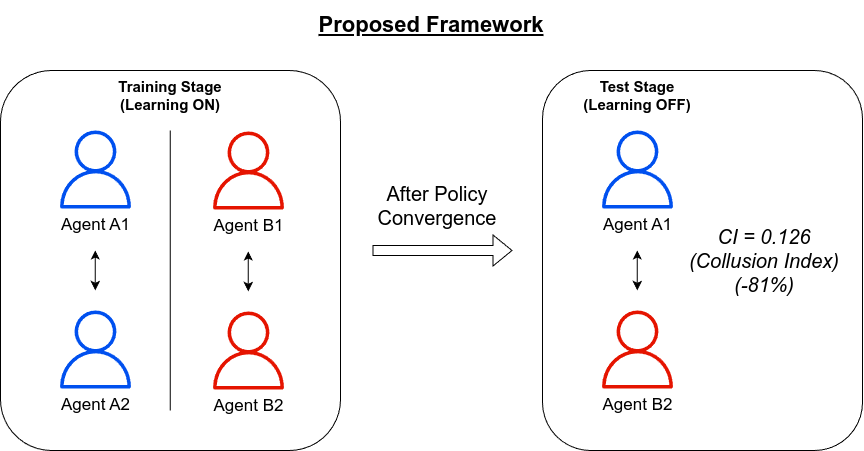
\includegraphics[keepaspectratio,alt={The stranger test: Calvano et al.'s rematching confined to the test stage, with learning off. Training is identical to Calvano et al.'s, replicated in independent runs (run A, run B); the manipulation is confined to the test stage: pairing an agent from run A with an agent from run B it never interacted with. If co-training produced individual collusive strategies, coordination would survive the re-pairing; if it produces a dyad-specific joint basin, it collapses. It collapses: CI falls from 0.674 (within-pair, Figure 1) to 0.126 (81\%; Section 4.4).}]{fig_framework_cross.png}}
\caption{The stranger test: Calvano et al.'s rematching confined to the
test stage, with learning off. Training is identical to Calvano et
al.'s, replicated in independent runs (run A, run B); the manipulation
is confined to the test stage: pairing an agent from run A with an agent
from run B it never interacted with. If co-training produced individual
collusive strategies, coordination would survive the re-pairing; if it
produces a dyad-specific joint basin, it collapses. It collapses: CI
falls from 0.674 (within-pair, Figure 1) to 0.126 (\ensuremath{-}81\%;
Section 4.4).}
\end{figure}

\subsection{Environment, training, and
protocols}\label{environment-training-and-protocols}

\textbf{Environment and training.} Bertrand-logit duopoly as in Section
2, 15-point grid spanning the Nash and monopoly benchmarks. Agents are
trained in pairs (``co-trained'') for 2M steps. Each run produces one
co-trained pair. The core population is 18 pairs; a post-hoc seed audit
found one run bit-identical to another (a resume-dependent seed formula
in the runner, since fixed), so statistics use the 17 unique pairs;
after the fix, retraining and six further runs extended the population
to 24 unique pairs, and results that use the extended population say so
explicitly. The exact-DP audit of Section 4.5 adds a high-fidelity
10M-step reference pair (38 agents in total). All post-training
evaluations are greedy (no learning, no exploration). Deliberate
divergences from Calvano et al.'s protocol (a fixed 2M-step budget with
10,000-step episode resets and random initial states, versus their
infinite horizon and 100,000-period stability criterion) are controlled
for by a separate five-pair population trained under the faithful regime
(no resets, single horizon, stability stopping rule), on which Section 5
reruns the entire audit chain. In total the paper draws on 24 co-trained
pairs at 2M steps, one 10M-step reference pair, five pairs under the
faithful regime, and 20 seeds per grid size in the granularity sweep of
Section 4.6; every audit is computed exactly on the converged policies,
pair by pair, rather than averaged over sessions.

\textbf{Reproducibility.} The environment, agents, training and audit
scripts, configurations, seeds and the converged Q-tables behind every
figure are available at
\url{https://github.com/kauelopes/algorithmic-collusion-without-deterrence}.

\textbf{Protocols.} (i) \emph{Impulse response}: after the pair settles,
one agent's price is exogenously forced for one period and both prices
are recorded over a {[}\ensuremath{-}5, +40{]} window; shocks go
\emph{down} (to the static best response, Calvano et al.'s deviation)
and \emph{up} (to the monopoly price); each cell runs under two arms,
co-trained and a \emph{cross-paired} control, with 10 random
initializations per pair. (ii) \emph{Fixed-opponent evaluation}: each
trained agent plays nine scripted strategies; a dedicated opponent-model
test initializes the joint state at the cooperative price, so that
trigger strategies start untriggered, and plays each agent 200 periods
against grim-trigger, constant-Nash and constant-monopoly opponents.
(iii) \emph{Cross-deployment}: agents from different runs are matched
and evaluated greedily. (iv) \emph{Exact dynamic programming}: fixing
the partner's greedy policy induces a 225-state MDP; we compute the
exact value of converged play and of the optimal best response; the
partner \emph{reacts}, so this is not a one-shot counterfactual. (v)
\emph{Null model}: the impulse-response protocol applied to pairs of
random Q-tables drawn on the same value range. (vi) \emph{Capacity
control}: hand-constructed punishment policies embedded in the same 225
\ensuremath{\times} 15 matrix.

\section{Results}\label{results}

\subsection{The phenomenon replicates}\label{the-phenomenon-replicates}

Everything we go on to audit, we first reproduce. Across 50 seeds at 2M
steps, the mean collusion index is \textbf{CI = 0.6245} (CI = 0 at the
Nash price, 1 at the monopoly price), within the range spanned by
published replications; a single high-fidelity run at 10M steps yields
CI = 0.6421 (the two use different grid widths, 1.0 for the 50-seed
batch and Calvano's 0.1 for the reference run, so the two indices are
not directly comparable). Our environment reproduces the phenomenon we
set out to examine. One number recorded here becomes important later: in
every run of this project in which it is measured on the converged
attractor (147 runs), the counterfactual deviation gain (CE-gap) is
strictly positive (0.014--0.082). No converged profile is free of an
incentive to deviate.

\subsection{The punishment pattern reproduces within the
pair}\label{the-punishment-pattern-reproduces-within-the-pair}

We first run Calvano et al.'s own test. Within co-trained pairs, a
forced one-period undercut produces exactly the published pattern: the
rival's price falls (mean drop 0.430 from a pre-shock level of 1.785),
and in 16 of 18 pairs both prices return \emph{exactly} to the
pre-deviation level, within about five periods (Figure 3, top-left). The
impulse-response evidence in Calvano et al. is not an artifact of their
code or ours; it is a robust property of co-trained Q-learning pairs in
this environment. The question is what it is evidence \emph{of}.

\begin{figure}
\centering
\pandocbounded{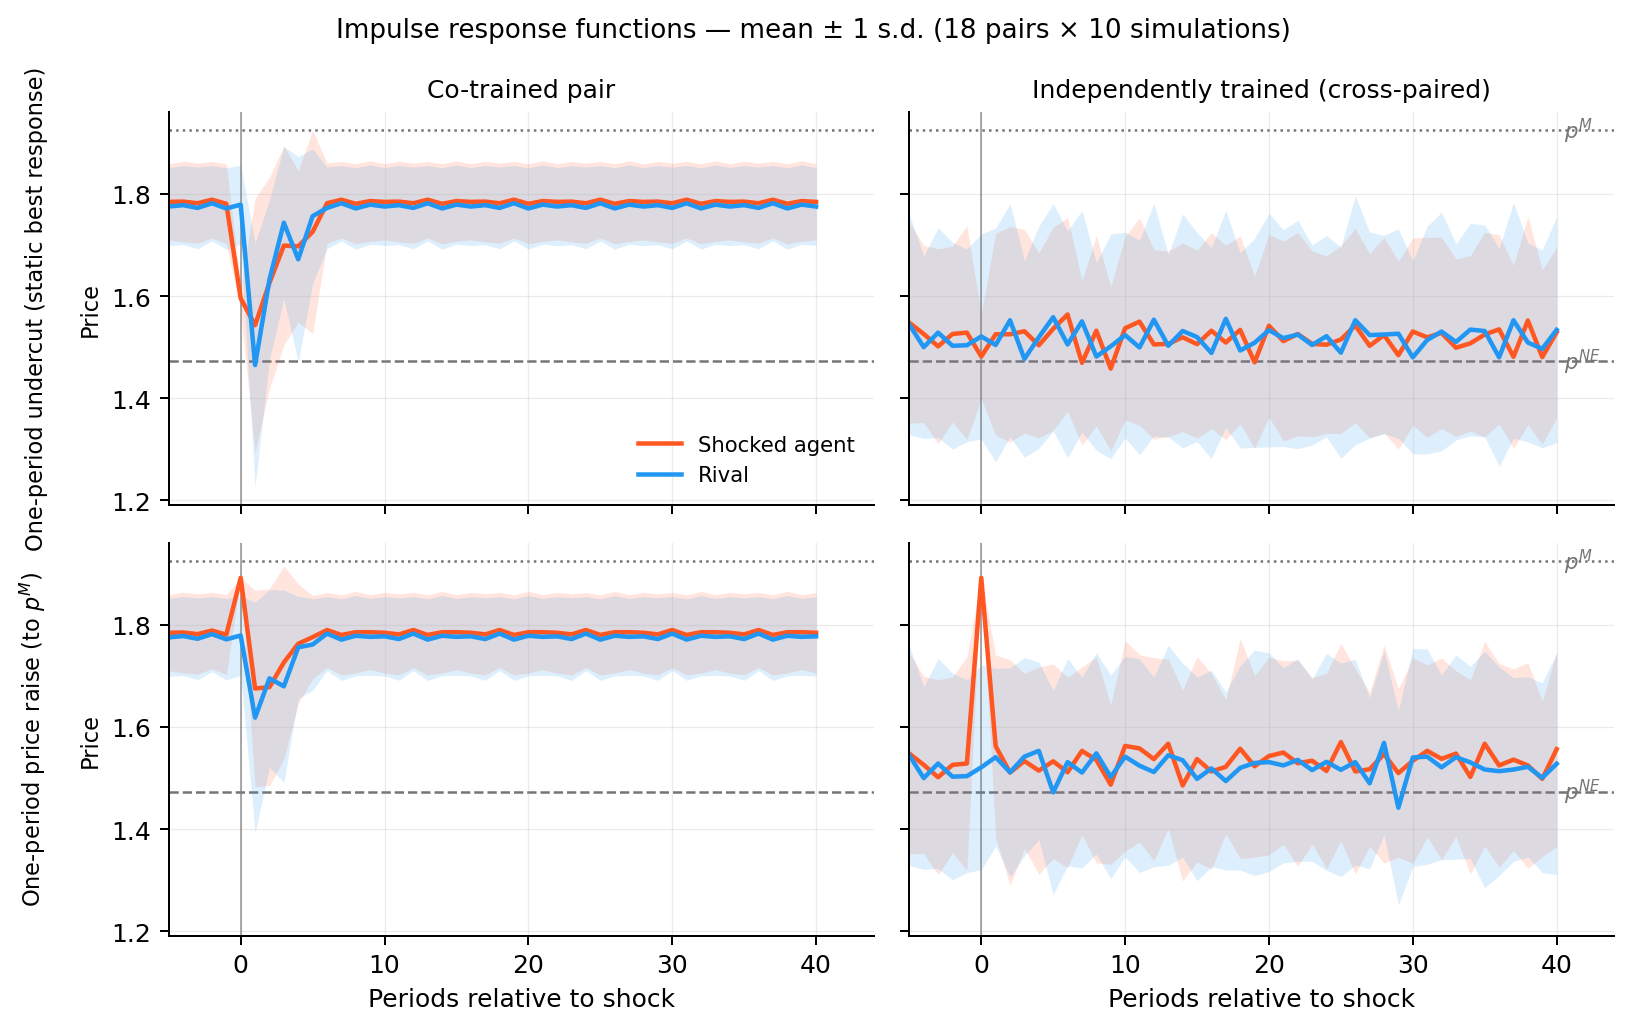
\includegraphics[keepaspectratio,alt={Impulse-response functions, mean  1 s.d. Rows: downward shock (static best response) and upward shock (to p\^{}M); columns: co-trained pair vs cross-paired control. Within pairs (left), both shocks produce the drop-and-return pattern; across pairs (right), the shock is invisible against the ambient variation.}]{fig_irf.png}}
\caption{Impulse-response functions, mean \ensuremath{\pm} 1 s.d. Rows:
downward shock (static best response) and upward shock (to p\^{}M);
columns: co-trained pair vs cross-paired control. Within pairs (left),
both shocks produce the drop-and-return pattern; across pairs (right),
the shock is invisible against the ambient variation.}
\end{figure}

\subsection{Auditing the mechanism}\label{auditing-the-mechanism}

A punishment scheme, in the sense of Section 2, has a signature: it
responds to departures from a prescribed path, it tracks the opponent it
is meant to discipline, and it makes deviating unprofitable. This
section tests the converged policies for each element of that signature,
in increasing order of severity: the response carries no information
about \emph{what} it is reacting to (i); it is insensitive to
\emph{whom} it is playing against (ii); the off-path policy has no
best-response structure to carry a threat (iii); the celebrated return
dynamic is over-determined rather than selective (iv), the pivotal test,
because with a single global attractor the exhibit would follow any
perturbation; and none of this is a representational limit, because
hand-built punishment rules fit the same matrix exactly (v).

\textbf{(i) The response carries no directional information.} This test
reproduces, in our population, the finding of \citet{epivent2024}, who
show in the same environment that price hikes are followed by the same
price wars as price cuts. A trigger rule may legitimately react to any
departure from the prescribed path, upward included, so a response to a
cooperative shock does not by itself refute path enforcement. The
information is in the \emph{form} of the response. When the forced shock
goes \emph{up} (the shocked agent raises its price to p\^{}M), the rival
responds with the same qualitative pattern as after an undercut: a drop
below baseline (to \ensuremath{\approx} 1.62 against a base of 1.78)
followed by the same return (Figure 3, bottom-left). Nothing in the
response encodes the direction, the payoff relevance, or the identity of
the perturbation. A response that treats a move toward the cartel price
exactly like a defection is consistent with basin relaxation; it is not
the signature of a rule whose function is to deter defection. Epivent
and Lambin note that such a rule is admissible in equilibrium but has no
counterpart in documented human collusion, and that on a grid shifted
below Nash the same agents punish upward moves toward Nash; what the
remaining audits add is that it is also not what the learned policy
carries.

\textbf{(ii) There is no working model of the opponent.} If the trained
agents carried a contingent retaliation rule, an opponent that actually
punishes (grim trigger) should elicit different play than an opponent
that never reacts (constant Nash). Designing this comparison requires
care: started from a random state, a grim rule reads the initial price
as a defection and reverts to Nash at once; the two opponents are then
behaviorally identical, and identical play against them proves nothing.
The valid design initializes the joint state at the cooperative price,
so the punisher starts cooperative. The result is sharper than mere
blindness: \textbf{22 of 24 trained agents undercut the grim punisher
within four periods}, triggering the permanent reversion its rule
announces, and never re-cooperate. The agents destroy a cooperative
arrangement that an opponent stands ready to enforce (Figure 4). In the
broader nine-strategy battery (complete over all 24 unique seeds), mean
CI against fixed opponents falls to 0.146, against 0.62--0.70 for the
same Q-tables with their training partners; and within every seed the CI
against nash, grim, wsls and imitation is identical, expected once the
punisher is triggered and symptomatic all the same.

\begin{figure}
\centering
\pandocbounded{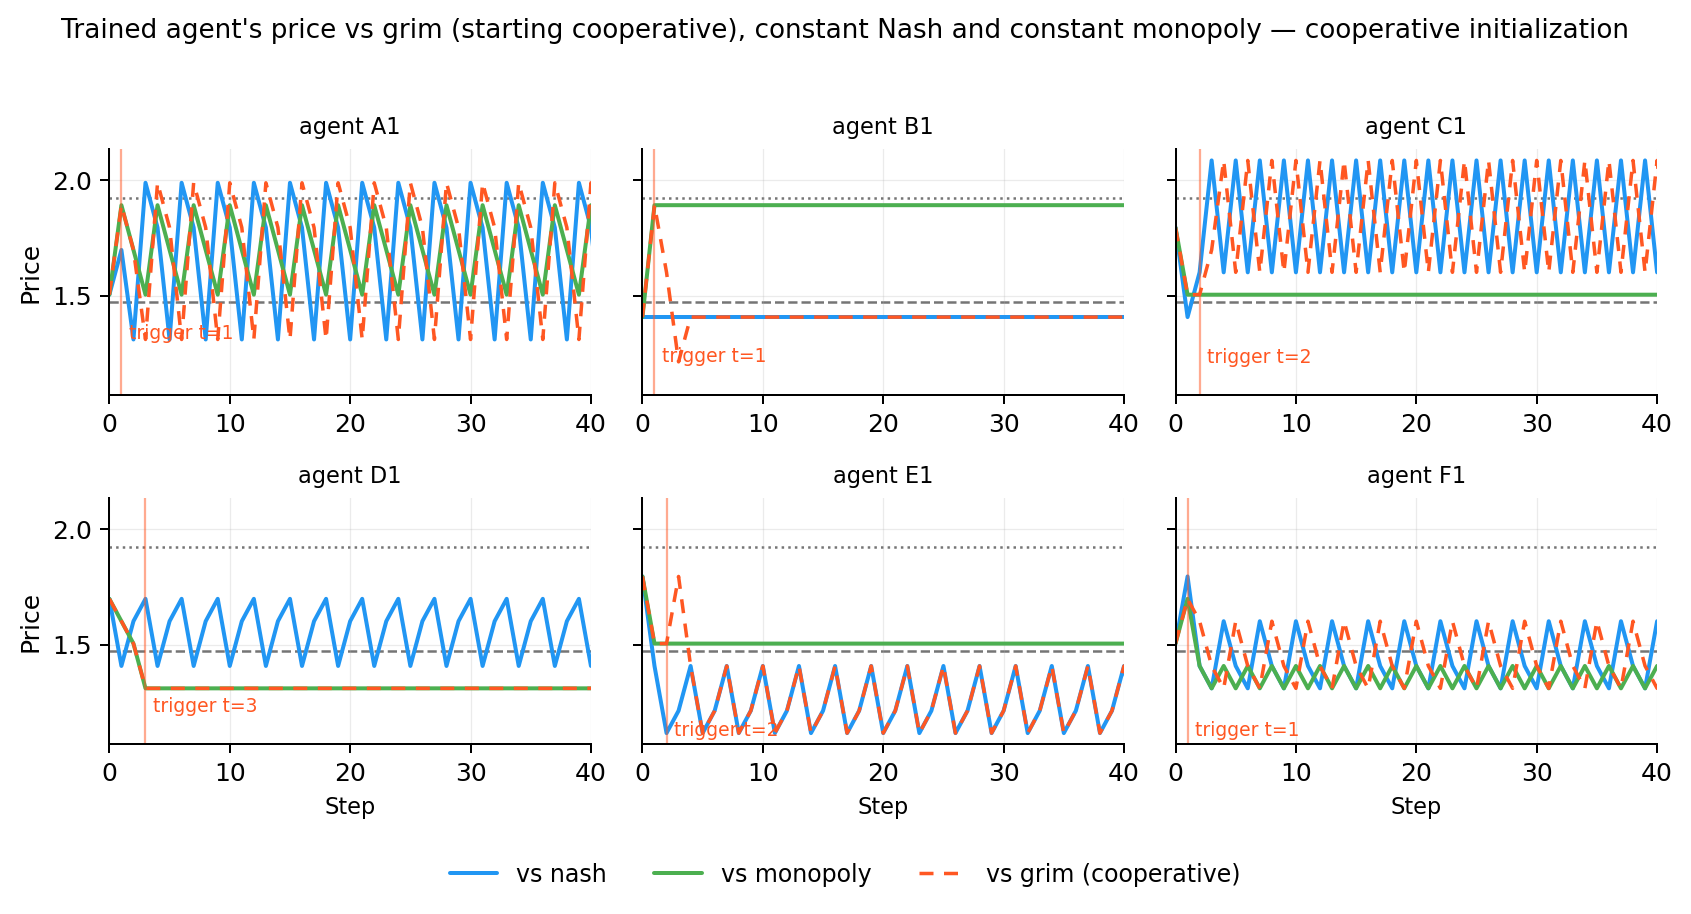
\includegraphics[keepaspectratio,alt={Trained agent's price path against a grim-trigger punisher started cooperative (dashed red), a constant-Nash pricer (blue) and a constant-monopoly pricer (green), from a cooperative initial state; six of the 24 agents shown, one panel per independent training pair (letters A--F), first agent of each pair. Vertical lines mark the period in which the agent's own undercut triggers grim's permanent reversion (22 of 24 agents, t  4).}]{fig_grim_vs_nash.png}}
\caption{Trained agent's price path against a grim-trigger punisher
started cooperative (dashed red), a constant-Nash pricer (blue) and a
constant-monopoly pricer (green), from a cooperative initial state; six
of the 24 agents shown, one panel per independent training pair (letters
A--F), first agent of each pair. Vertical lines mark the period in which
the agent's own undercut triggers grim's permanent reversion (22 of 24
agents, t \ensuremath{\leq} 4).}
\end{figure}

\textbf{(iii) There is no best-response logic off-path.} The learned
policy is a 225-entry lookup table we can inspect directly. Slicing each
agent's policy at its on-path price yields its \emph{reaction function}:
price at t as a function of the rival's price at t\ensuremath{-}1.
Against the clean, monotone static best-response curve, the 18 learned
reaction functions are noise: mean Spearman \ensuremath{\rho} =
\textbf{0.016} (range {[}\ensuremath{-}0.47, 0.52{]}). The full policy
heatmaps are salt-and-pepper over the entire state space; the only
economically interpretable point is the on-path attractor itself.

\textbf{(iv) The return is over-determined, not selective.} Here is the
pivotal step. Under this state representation, the state \emph{is} the
previous joint action; two fixed greedy policies therefore define a
deterministic map on 225 states, and by the pigeonhole principle every
orbit is eventually periodic. Reaching \emph{some} cycle is guaranteed
by the object class; the question is whether a rule selects the
destination or the map leaves nowhere else to go. Enumerating the full
state space settles it: \textbf{17 of 18 trained pairs have exactly one
attractor whose basin is all 225 states} (mean dominant-basin share
99.9\%, mean 1.06 attractors per pair), and the exact-return rate after
a forced deviation is \textbf{100\% (90/90 trials)}. This is the
structural reason for (i): with one globally attracting cycle, the orbit
after a defection and the orbit after a cooperative shock cannot differ.
A random-policy null locates the behavior: random Q-tables drawn on the
same value range fragment the space (3.26 attractors, dominant basin
79.2\%, Mann--Whitney p = 6.3 \ensuremath{\times} 10\ensuremath{^{-8}})
and return only \textbf{62.0\%} of the time (310/500, Fisher p = 1.8
\ensuremath{\times} 10\ensuremath{^{-17}}), so the global basin is not a
property of the state space alone. What training adds is \textbf{speed
and placement}: 3.62 steps to return against 13.87 (p = 5.8
\ensuremath{\times} 10\ensuremath{^{-32}}), and 96.7\% of returns land
at CI \textgreater{} 0.3 against 62.6\% for random pairs (Figure 5).
Speed and placement without selectivity are calibration, not deterrence:
the trained pair returns to its path from anywhere and for any reason,
which is what a basin does and not what a trigger rule does.

\begin{figure}
\centering
\pandocbounded{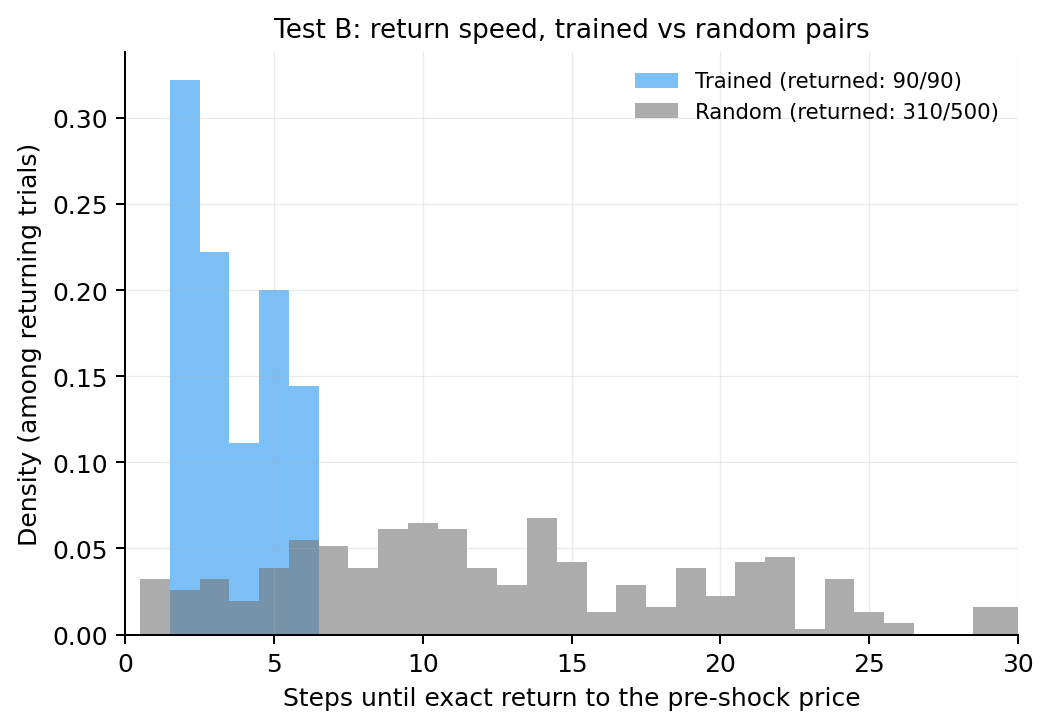
\includegraphics[keepaspectratio,alt={Null model, return speed: steps until exact return to the pre-shock price, among returning trials. Trained pairs (blue) return in 3.62 steps on average and in 90 of 90 trials; random Q-table pairs (gray) take 13.87 steps and return in 310 of 500 (62.0\%). Fisher p = 1.8  10 on the rates, Mann--Whitney p = 5.8  10 on the speed; the basin shares (99.9\% vs 79.2\%) are reported in the text.}]{fig_null_model_return_rate.png}}
\caption{Null model, return speed: steps until exact return to the
pre-shock price, among returning trials. Trained pairs (blue) return in
3.62 steps on average and in 90 of 90 trials; random Q-table pairs
(gray) take 13.87 steps and return in 310 of 500 (62.0\%). Fisher p =
1.8 \ensuremath{\times} 10\ensuremath{^{-17}} on the rates,
Mann--Whitney p = 5.8 \ensuremath{\times} 10\ensuremath{^{-32}} on the
speed; the basin shares (99.9\% vs 79.2\%) are reported in the text.}
\end{figure}

\textbf{(v) The absence is not architectural.} One might object that a
225-state lookup table cannot express punishment, making its absence
trivial. We check this by construction. We hand-build two policies in
the identical 225 \ensuremath{\times} 15 matrix, with the same state
indexing as the trained agents: a reactive rule (play Nash whenever the
rival's last price was below a threshold, otherwise cooperate, so
punishment lasts as long as the deviation and is then forgiven) and a
grim rule (the same trigger, but once the agent's own last price is Nash
it stays at Nash, so its own past price serves as a phase flag and the
punishment is permanent). Simulated in the same environment against a
scripted rival that cooperates, undercuts to the grid minimum for five
periods and returns, from a cooperative initial state, the reactive
policy punishes for exactly the five periods of the deviation and
returns with the rival, and the grim policy punishes and never returns
(Figure 6). Their policy heatmaps show the threshold structure as clean
bands, in direct contrast with the salt-and-pepper learned policies. The
representational capacity is there; the learning process did not use it.

\begin{figure}
\centering
\pandocbounded{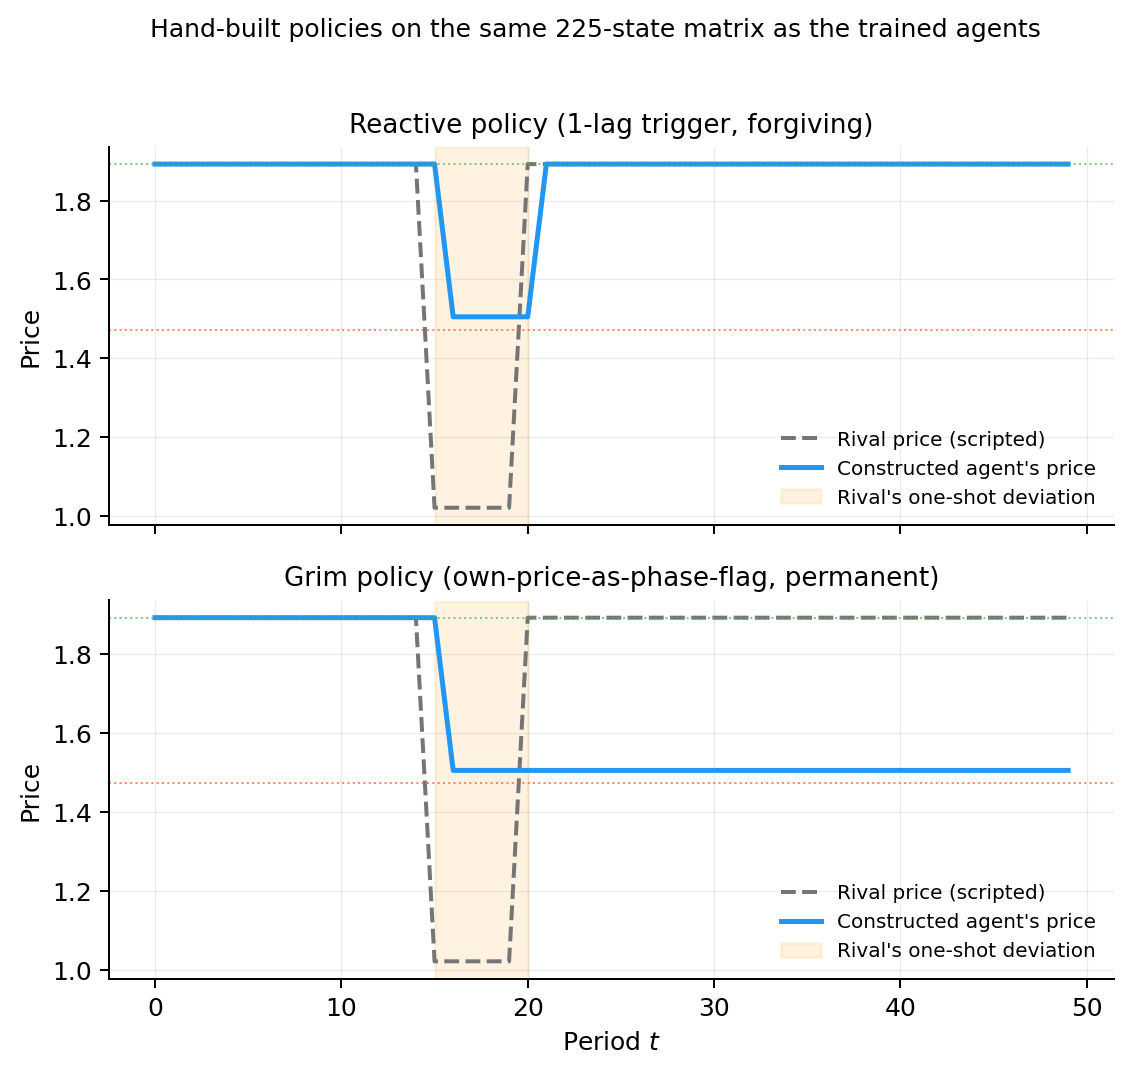
\includegraphics[keepaspectratio,alt={Capacity control: hand-built policies in the same 225  15 matrix as the trained agents, simulated in the same environment against a scripted rival that undercuts for five periods (shaded) from a cooperative joint state. Top: the reactive rule punishes for the duration of the deviation and forgives. Bottom: the grim rule, using its own past price as a phase flag, punishes permanently. Dotted lines mark the Nash and cooperative prices.}]{fig_constructive_punishment_trajectories.png}}
\caption{Capacity control: hand-built policies in the same 225
\ensuremath{\times} 15 matrix as the trained agents, simulated in the
same environment against a scripted rival that undercuts for five
periods (shaded) from a cooperative joint state. Top: the reactive rule
punishes for the duration of the deviation and forgives. Bottom: the
grim rule, using its own past price as a phase flag, punishes
permanently. Dotted lines mark the Nash and cooperative prices.}
\end{figure}

\subsection{The dyad is the unit: nothing survives outside the
pair}\label{the-dyad-is-the-unit-nothing-survives-outside-the-pair}

If what training produces is a pair-specific basin rather than
individual strategies, coordination should not survive rematching, just
as, in partner-to-stranger comparisons in the laboratory, behavior that
is a personal norm travels and behavior that is a pair-specific
convention does not. \citet[Section VI.B]{calvano2020} ran this rematch
with learning on and saw profit gains fall from 85\% to about 20\%
before re-learning partially restored them; with learning off, the
collapse is the whole story. Agents trained under identical protocols
but in different runs, when cross-matched and evaluated greedily,
collapse from within-pair \textbf{CI = 0.674 to CI = 0.126}, an 81\%
loss (12 cross-matchings, all unique after the seed audit); in an
extended combinatorial evaluation (40 matchings), mean CI is 0.109 and
\textbf{30\% of matchings price below Nash} (Figure 7). The cross-paired
impulse response makes the point visually: there is no plateau to
defend, prices hover noisily around p\^{}NE, and the forced deviation is
invisible against the ambient variation (Figure 3, right column). In
machine-learning terms, this is an out-of-distribution failure: each
policy was fit to the distribution of states its particular partner
generates, and a new partner, even one trained under an identical
protocol, moves the test distribution. The pair has overfit to itself.
Collusion in this environment is not a strategy an agent \emph{has}; it
is a convention a pair \emph{keeps}.

\begin{figure}
\centering
\pandocbounded{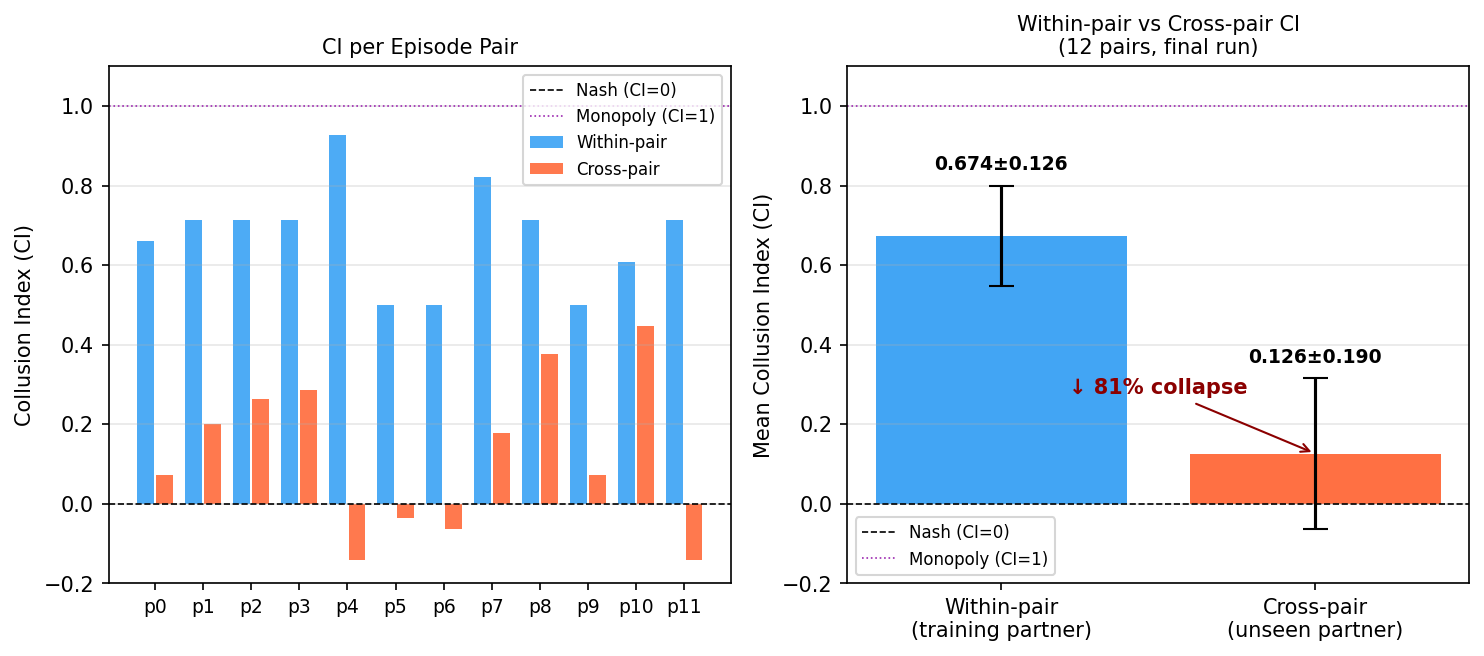
\includegraphics[keepaspectratio,alt={Within-pair vs cross-pair collusion index, per matching: CI collapses from 0.674 to 0.126 (81\%) when independently trained agents are cross-matched (12 matchings).}]{fig_cross_deploy_ci_comparison.png}}
\caption{Within-pair vs cross-pair collusion index, per matching: CI
collapses from 0.674 to 0.126 (\ensuremath{-}81\%) when independently
trained agents are cross-matched (12 matchings).}
\end{figure}

\subsection{What is deterred, and what is
not}\label{what-is-deterred-and-what-is-not}

\textbf{Deterrence-in-effect holds for the deviation Calvano et
al.~test.} We first run their own profitability calculation on our
pairs: given what the rival actually does after the forced one-period
undercut, does the deviation pay? It does not, in \textbf{18 of 18
pairs}: the one-period gain (mean +0.040) is outweighed by the
discounted losses of the post-deviation phase (mean
\ensuremath{-}0.240), for a mean net of \textbf{\ensuremath{-}0.200}
(\ensuremath{\delta} = 0.95). On this point we replicate Calvano et
al.~exactly.

\textbf{But the deterred deviation is not the relevant one.} The
positive CE-gap of Section 4.1 can be made concrete. Fixing each
partner's actual greedy policy and solving the induced 225-state MDP
exactly (\ensuremath{\delta} = 0.95), the optimal best response, against
a partner who \emph{reacts}, improves on converged discounted profit by
\textbf{14.8\% on average} (median 12.8\%, maximum 48.0\%; 10 of the 38
agents are at an exact best response, and excluding the duplicated pair
the figures are 15.6\%, 13.4\% and 8 of 36) (Figure 8). This is a
demanding test (no learning agent computes exact DP), and we use it not
to demand optimality but to size the wedge: the profile leaves, on
average, a seventh of the achievable payoff on the table against the
very partner it converged with. The juxtaposition resolves the apparent
tension: what the converged dyad deters is the \emph{naive} deviation, a
single-period undercut followed by a return to the old policy, which is
precisely the deviation no optimizer would choose; the \emph{optimal}
deviation policy, which anticipates the partner's reaction, profits by
14.8\%. Neither agent ever samples the deviations that would profit it.
The supracompetitive prices are not \emph{enforced}; they are merely
\emph{undisturbed}: collusion survives because deviation is never tried,
not because it would not pay. This also locates our measure relative to
the \emph{Q-loss} of \citet[Section III.D]{calvano2020}, who evaluate
each limit strategy against the rival's and report about half of their
sessions in on-path Nash equilibrium, with a mean on-path Q-loss of
0.2\%. As we read their procedure, the Q-loss is the forfeited payoff of
a one-step improvement under the agent's own continuation, checked at
on-path states; our wedge is the value of the full optimal policy from
the converged state, which may leave the path and keep deviating. The
two are consistent: no profitable one-step deviation on path, a
profitable plan off it, which is the sense in which the path is
undisturbed rather than enforced. In the vocabulary of Calvano IJIO and
of the survey by \citet{tang2024}, the deterrence is \emph{incomplete}:
genuine with respect to the one-period deviation they test, and spurious
with respect to the optimal one, in Calvano IJIO's own sense of prices
sustained by not recognizing the gain from deviating. We therefore do
not claim that retaliation plays no stabilizing role against naive
deviations; we claim that the role it plays does not extend to the
deviation an optimizer would choose, which is the one that decides
whether the path is enforced.

\begin{figure}
\centering
\pandocbounded{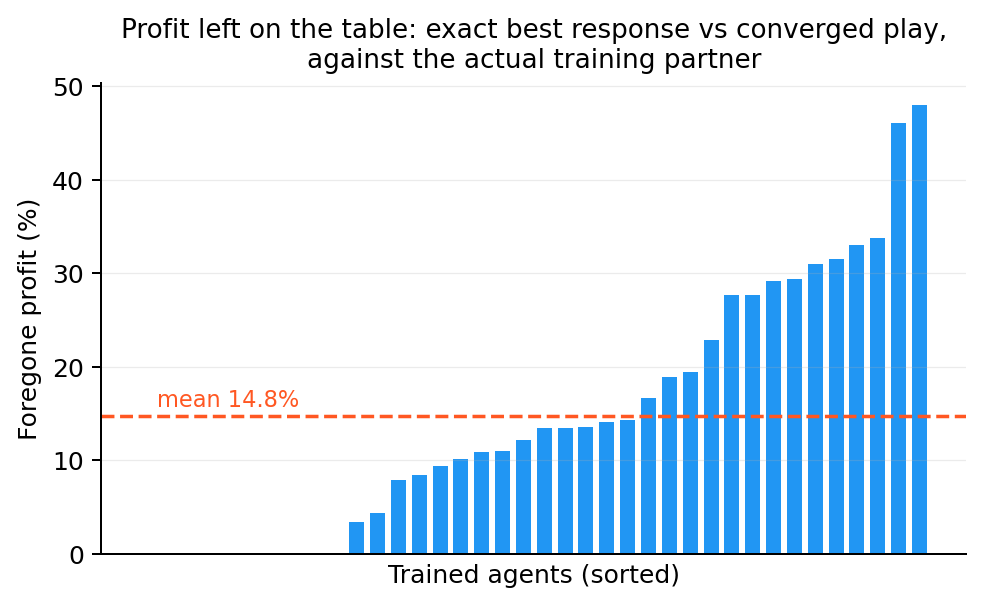
\includegraphics[keepaspectratio,alt={Exact best-response gain over converged play, per agent (38 agents): mean 14.8\%, median 12.8\%, maximum 48.0\%; 10 of 38 agents are at an exact best response.}]{fig_ce_gap_interpretable.png}}
\caption{Exact best-response gain over converged play, per agent (38
agents): mean 14.8\%, median 12.8\%, maximum 48.0\%; 10 of 38 agents are
at an exact best response.}
\end{figure}

\subsection{Why: the visitation funnel}\label{why-the-visitation-funnel}

One mechanism explains both halves of the results (why the audit finds
no scheme, and why nothing survives outside the pair), and it is visible
in training. As \ensuremath{\varepsilon} decays, state--action
visitation concentrates on a narrow neighborhood of the joint
trajectory; off-path entries of the Q-tables retain their initialization
values or reflect a handful of samples. The policy outside the basin is,
in the operative sense, untrained, which is why it behaves like the
random-map null model wherever the basin's local calibration runs out.

The funnel makes a comparative-statics prediction: enlarging the state
space, by refining the price grid, spreads the same exploration budget
over more off-path states and should weaken coordination. The prediction
holds. Holding the training budget at 2M steps and varying the grid from
5 to 200 points (20 seeds per level), mean CI declines monotonically
from 0.74 (5 points) and 0.74 at Calvano's 15, to 0.64 (50), 0.59 (100)
and 0.43 (200 points), consistent with the granularity sensitivity in
\citet{klein2021}, and prices remain supracompetitive even at the finest
grid (Figure 9). The basin account thus predicts evidence beyond the
audit it was built to explain. And the same exploration decay that
stabilizes the collusive path removes the experience that would test it:
the funnel builds the basin and then seals it.

\begin{figure}
\centering
\pandocbounded{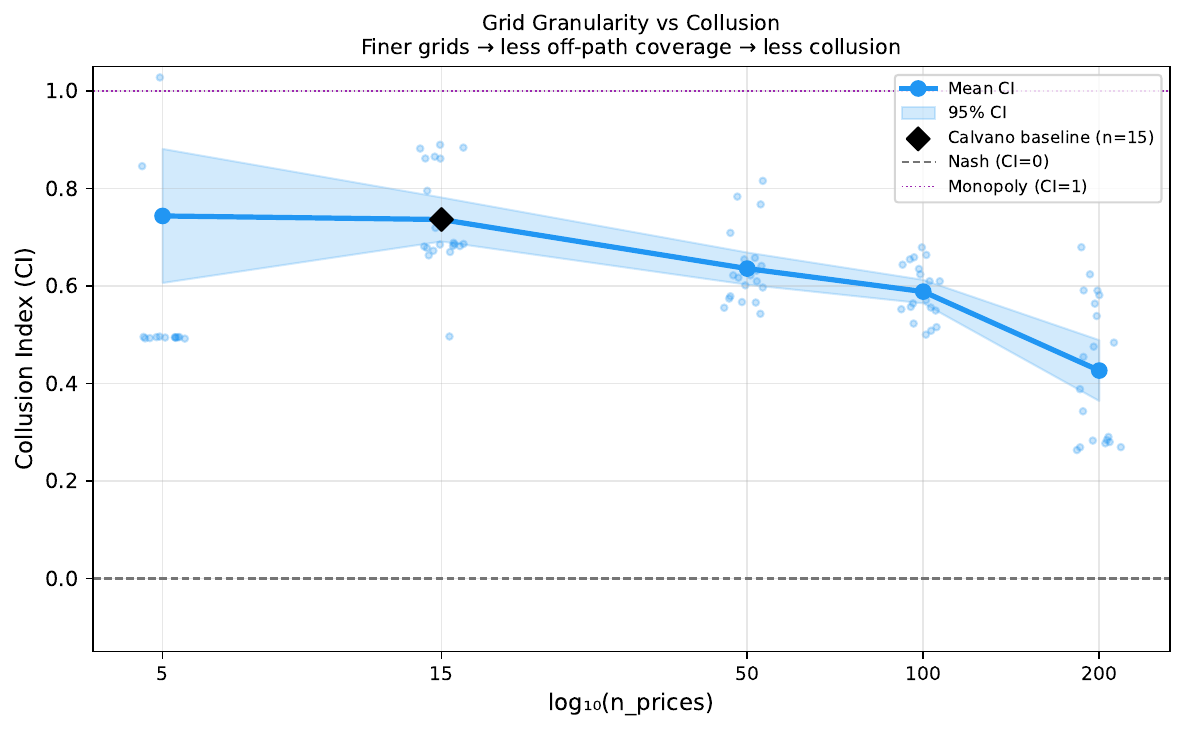
\includegraphics[keepaspectratio,alt={Grid granularity: mean CI (20 seeds per level, 2M steps) declines monotonically as the price grid is refined from 5 to 200 points; the black diamond marks Calvano's 15-point baseline.}]{fig_grid_sensitivity_ci.png}}
\caption{Grid granularity: mean CI (20 seeds per level, 2M steps)
declines monotonically as the price grid is refined from 5 to 200
points; the black diamond marks Calvano's 15-point baseline.}
\end{figure}

\section{Discussion}\label{discussion}

\textbf{What the evidence supports.} The converged objects in this
environment are not individual pricing strategies sustained by
contingent retaliation. They are two halves of a jointly carved
attractor: fast and stable at home, structureless everywhere else. None
of the signatures of a punishment scheme we test for is present, while
the capacity control confirms the architecture could have expressed
them. The natural theoretical name for this object is a
\emph{self-confirming equilibrium} \citep{fudenberg1993}: each agent's
beliefs are correct on the realized path and never tested off it, so
play is optimal against beliefs that no experience contradicts, without
being optimal against the opponent's actual strategy. We offer this as
an interpretation, not a theorem. The dynamics that produce such an
object have a candidate description in \citet{banchio2022}, in a
stateless setting: the value estimates of co-learning agents are
correlated through the joint action, and the correlation, not any
threat, holds the profile together; the self-confirming equilibrium is
what that coupling leaves behind once exploration stops. Our capacity
control speaks to their conjecture that memory, by enabling
reward--punishment strategies, would substantially increase collusion:
with one period of memory the capacity is present and unused. We also
follow \citet{denboer2022} in preferring the language of optimality to
that of threats: algorithms are neither tempted nor deterred, and asking
whether a converged policy is a best response to its partner, as Section
4.5 does, is the question that remains well posed once that vocabulary
is set aside. Put in Lucas-critique terms: the learned rule is
calibrated to one particular environment, and here the partner \emph{is}
the environment; change the partner and the rule loses its object.

\textbf{Reconciling with \citet{calvano2023}.} Calvano IJIO verify
approximate incentive compatibility on their converged profiles; our
exact-DP audit finds mean best-response gains of 14.8\%, even though the
single-deviation profitability test of the 2020 paper \emph{replicates}
on our pairs (Section 4.5). To rule out the training regime as the
explanation, we retrained five pairs to Calvano's own stopping rule (no
episode resets, single horizon, policy stable before termination) and
reran the entire audit chain. Every result survives: the
impulse-response pattern reproduces in 5 of 5 pairs, the cooperative
grim punisher is undercut by 4 of 5 agents (the fifth never triggers
it), the one-period deviation remains unprofitable in 5 of 5, and the
exact best response still gains \textbf{10.4\% on average}. Training to
convergence \emph{narrows} the incentive wedge, from 14.8\% to 10.4\%,
but does not close it. The remaining divergence from the ``genuine
collusion'' classification lies primarily in the deviation class checked
(one-period undercut versus exact dynamic best response), not in the
training regime.

\textbf{Implications for the literature and for policy.} The
impulse-response figure has served as the literature's strongest exhibit
for treating learned supracompetitive pricing as collusion in the
legal-economic sense. Our results do not overturn the figure; they
reinterpret it. A drop-and-return after any perturbation is what a
policy pair with a single global attractor does; its evidentiary value
for \emph{deterrence} is small without the controls run here. Studies
inferring mechanisms from on-path behavior alone risk attributing to
strategy what is, mechanically, basin geometry. The consumer-welfare
concern, however, is not dissolved: prices are robustly supracompetitive
(CI \ensuremath{\approx} 0.62--0.70 within pairs), and that harm is
unchanged by anything in our audit. What changes is the remedial
reading. The ``strategy'' does not transfer to any opponent not present
during training, including opponents strictly more cooperative than the
training partner; and the absence of a contingent scheme cuts
\emph{against} mapping the dyad onto agreement-like legal categories (a
meeting of minds enforced by threats). Our evidence licenses only a
frozen-policy claim: disturbing the pairing (entry, rotation,
retraining) destroys coordination among the converged policies we study.
\citet[Section VI.B]{calvano2020} show that continued learning does
re-carve a basin after recomposition, over tens of thousands of further
periods; what our data add is that nothing is carried into that process
by the policies themselves. The absence of a contingent scheme does not
shrink the enforcement problem; it relocates it, from detecting threats
that are not there to disturbing pairings that re-form only at the cost
of re-learning at live prices, a cost the frozen test shows starts from
zero coordination.

\textbf{Implications for machine-learning pricing at large.} Pricing
decisions are increasingly delegated to learning systems, and the field
evidence shows the stakes are not hypothetical: algorithm adoption
measurably changes price competition \citep{brown2023, assad2024}. For
that setting our results carry a warning and a toolkit. The warning is
methodological: any claim that deployed pricing agents have learned to
coordinate, or to punish, inherits the evaluation problem documented
here, because market data record only the on-path behavior of one
particular grouping of algorithms, and Section 4 shows that on-path
behavior alone cannot identify a mechanism. The same caution applies
inside firms and platforms: a pricing system that performs well against
the agents it was trained or tuned with has demonstrated a property of
the \emph{ensemble}, not of the policy; our cross-pairing result is a
measured example of how large that gap can be. The toolkit is the audit
itself: every protocol used here (stranger re-matching, directional
shocks, opponents with explicit rules, random-policy null models,
exploitability accounting) is defined on frozen policies and portable to
any multi-agent pricing stack, including deep RL systems. Together they
form a pre-deployment evaluation standard for a question that on-path
monitoring cannot answer: whether apparent coordination is a strategy
the agent carries, or a property of the ensemble that trained together.

\textbf{Limitations.} (1) \emph{Population}: the core population is 17
unique co-trained pairs (one run of 18 was excluded as a bit-identical
duplicate after a seed audit; the corrected runner later extended the
population to 24 unique pairs, used where stated); the extended
combinatorial cross-evaluation covers 40 of the 153 possible matchings
(truncated in enumeration order, not sampled). (2) \emph{Statistics}:
the separation claims in Section 4.3(iv) are reported with pair-level
aggregation; the trained arm is at a ceiling (18 of 18 pairs at rate
1.000), so the pair-level variance is zero on one side, and the interval
on the rate difference, {[}+0.318, +0.442{]}, should be read as a floor
on the separation rather than a precise estimate. (3) \emph{Training
regime}: the main population trains a fixed 2M steps with episode resets
rather than to Calvano's stability criterion; the five-pair rerun under
the faithful regime replicates the entire audit chain, with the wedge
narrowing to 10.4\%; larger regime-faithful populations remain
desirable. (4) \emph{Scope}: our claims are about tabular Q-learning in
the Calvano environment, at its baseline parameterization (one demand
specification, one 15-point grid, \ensuremath{\delta} = 0.95), and they
are bounded by it. The protocol-level audits (up-shock, opponent
battery, cross-pairing) are portable to function-approximation agents;
the eventual-periodicity argument behind the null model is not (it is
specific to finite deterministic policy maps), and whether deep agents
learn genuinely contingent responses is an open question our protocol is
designed to answer, not presuppose. Within that scope, none of the
signatures of deterrence we test for is present, and what is present is
basin geometry.

\section{Conclusion}\label{conclusion}

We replicated the central exhibit of the algorithmic collusion
literature and asked the question the exhibit was taken to answer: is
there a punishment mechanism? None of five independent audits finds one.
The response to deviation carries no directional information; faced with
a punisher whose cooperation was there to be kept, the agents defect and
absorb the punishment; their reaction functions are uncorrelated with
best-response logic; their celebrated return-to-baseline is
over-determined, since 17 of 18 pairs have a single attractor covering
the whole state space; and none of this is explained by a
representational limit. What training produces instead is a
dyad-specific basin of attraction: re-match frozen agents from
independent runs and coordination collapses by 81\%, from CI = 0.674 to
0.126. And the path the basin holds is not incentive-compatible against
the optimal deviation, which, computed against each partner's frozen
strategy, profits by 14.8\% on average. The scheme deters only the
deviation no optimizer would choose. Collusion here is not a strategy
either agent has; it is a convention the pair keeps. This reading
unifies what the literature had measured separately: the
pair-specificity Calvano et al.~observed on rematching, the
direction-blind response Epivent and Lambin documented, the gap between
impulse patterns and equilibrium den Boer et al.~established, and the
punishment-free coupling Banchio and Mantegazza modeled.

The methodological point outlasts the specific exhibit. As pricing
migrates to learning systems, behavioral patterns produced by black-box
agents will increasingly reach regulators and courts as evidence of
algorithmic coordination, and such patterns invite mechanistic
over-reading: the drop-and-return \emph{looks} like retaliation, and
controls are what tell the difference. Mechanism claims about learned
behavior should be held to the standard applied here: survive an
explicit null, survive removal from the training context, survive an
incentive accounting. What the standard buys is precision about the
policy problem. The supracompetitive prices, and the harm they imply,
are robust; what is absent is the deterrence behind them, and harm and
mechanism call for different instruments: an outcome can be monitored,
but only an agent that carries a rule can be deterred. Prices in this
environment are high not because deviation is punished, but because,
once exploration has decayed, deviation is never tried, and the beliefs
that would motivate it are never corrected.

\bibliographystyle{ACM-Reference-Format}
\bibliography{refs}

\end{document}
